\documentclass{article}
\usepackage{graphicx}
%\usepackage{subfig}
\usepackage{amsmath}
\usepackage{mathtools}
\usepackage{cleveref}
%\usepackage{subfig}	
\usepackage{subcaption}
\usepackage[numbered,framed]{mcode}
\usepackage{fixltx2e}				% For the \textsubscript{} usage
\usepackage{textgreek}	

\author{Grupp B}
\title{FRT090 \\Feedback Seminar 1(Modeling/Design)  }				% \\ <=> NEW LINE IN LaTex
\date{November 2014}


\begin{document}
\maketitle	% prints the preamble onto the pdf
\newpage


\section {Overview over the project and its objectives}

Our system is a unicycle which will maintain the balance in two directions. The first being the pitch and the second being roll. It should maintain balance in realtime and withstand small disturbances meaning a small puch in the pitch or roll direction. The system is being divided into two parts, the first being the part which will maintain the balance in the roll direction. The realization will be a inverted pendulum with a inertia wheel at the top. While the balancing part in the pitch direction will be achieved with a wheel attached at the end of the inverted pendulum. In other words there will be two processes which will be regulated, the inverted pendulum  with the inertia wheel and the inverted pendulum with a wheel at the bottom. 



\section{Discussion on the modeling needs in the project}

\subsection{Why is modeling needed and what should models be used for}

The modeling part is essential to understand how the process acts, how the different physical quantities interact (how the velocity and acceleration for instances look like and what affect them). In our chase we need to design a wheel for the inertia but different dimensions will give different result but as engineers we want to maximize the effect we need without maximizing the negative effect on the objective of the design. So in essence we use models to design parts needed in the implementation. However there more models can be used for as to investigate how the robustness theoretically, investigate which regulator is suited for this specific process and simulate it for example. But most important to investigate the stability of the model thru some standard calculations (look at the transfer function which will give us the poles).   

\subsection{How is a model quality assessed}

The best way to find out the quality of the model is to simulate it and se if the result is reasonable with the expected result (in the easier cases if the process is to complex it is hard to predict the result). Make use of prior knowledge of similar processes.    


\section{Description of the models developed so far in the project }

% Equation describing 
\begin{equation}
		\begin{aligned}
	     	 (J_{w}+ML^2 + J_{p} ) \frac{\partial^2 \theta_{1} }{\partial t^2}  &= l_{1} \sin{\theta_{1}} m g + L \sin{\theta_{1}} M g - \tau    \\  
		 J_{w} \frac{\partial^2 \theta_{2}} {\partial t^2} &= \tau
		\end{aligned}
	 	\label{equ:inverted_pendulum}  
\end{equation}


The model we have so far is given in by equation \ref{equ:inverted_pendulum} which describes the inverted pendulum with the inertia wheel at the top. As one also can see in figure \ref{fig:sketch_inverted_pendulum} which is a sketch of the model so far. The rod is stationary while the inertia wheel can can spin around the axis of the rod at the top. So basically this is the process.

\begin{figure}
	\centering
	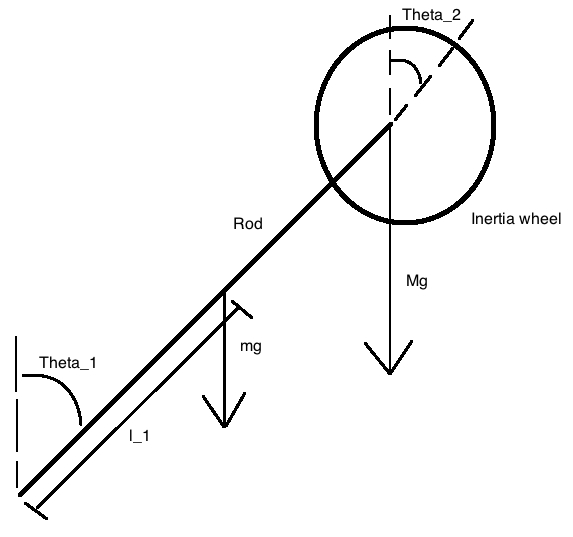
\includegraphics[width=0.7\textwidth]{Inverted_pedulum_2}
	\caption{Shows the sketch of the inverted pendulum and the meaning of the parameters.}
	\label{fig:sketch_inverted_pendulum}
\end{figure}



\section{Motivation for the selected modeling \& design approaches}

We choose to go with the Newton model which seems to be the most familiar model for us in the group due to prior knowledge with Newtons laws of forces and torques. There is other approaches which can be Lagrange's mechanics which is a essentially a statement derived from Newtons laws which simplify the work of describing more complex systems. Regarding the design approaches one would like to have some characteristics as fast response time, minimal overshoot and be able to handle disturbences for the process which can be achieved with a PID regulator. Luckily there is a way of specifying the demands and Simulink does the calculations of the parameters in the PID regulator. 


\section{Discussion on experience with respect to modeling and design}

The biggest experience was that one need to have a good model for the system to be able to find out how the process behaves and then simulate it in Simulink with Matlab to actually se where the pools are placed. But before simulating it one need to do some calculations by hand so one can compare the handwritten solution with the simulation. Because maybe in the process of simulating the process one can do mistakes, these mistakes are easy to find if one have a handwritten result to compare with.  

\end{document}